\documentclass{jsarticle}[12pt]
\usepackage{amsmath}
\usepackage{amsbsy} %%iranaippoi%%
\usepackage{amsthm}
\usepackage{amssymb}
\usepackage{amscd}
%%\usepackage{url}
\usepackage[top=25truemm,bottom=25truemm,left=25truemm,right=25truemm]{geometry}
\usepackage[utf8]{inputenc}
\usepackage[all]{xy}
\usepackage[dvipdfmx]{graphicx}
%%\usepackage[dvipdfm,citecolor]{hyperref}

\author{kamojiro @kamojiro24e}
\title{Notes on discrete groups and Furstenberg boundaries}

\theoremstyle{break}
\newtheorem{theorem}{定理}[section]
\newtheorem{corollary}{系}[theorem]
\newtheorem{definition}{定義}[section]
\newtheorem{proposition}{命題}[section]
\newtheorem{lemma}{補題}[section]
\newtheorem{remark}{注}[theorem]
\newtheorem{example}{例}

\renewcommand{\<}{\langle}
\renewcommand{\>}{\rangle}
\newcommand{\C}{\mathbb{C}}
\newcommand{\R}{\mathbb{R}}
\newcommand{\N}{\mathbb{N}}
\newcommand{\Z}{\mathbb{Z}}
\newcommand{\Q}{\mathbb{Q}}
\newcommand{\A}{\mathcal{A}}
\newcommand{\T}{\mathcal{T}}
\newcommand{\D}{\mathcal{D}}
\newcommand{\fN}{\mathfrak{N}}
\newcommand{\fM}{\mathfrak{M}}
\newcommand{\Tr}{\rm{Tr}}
\renewcommand{\O}{\mathcal{O}}
\newcommand{\F}{\mathbb{F}}
\renewcommand{\P}{\mathcal{P}}
\newcommand{\id}{{\rm id}}
\newcommand{\Axis}{{\rm Axis}}
\newcommand{\Aut}{{\rm Aut}}
\newcommand{\Fix}{{\rm Fix}}
\renewcommand{\d}{\frak{\partial}}
\renewcommand{\L}{\rm{L}}
\newcommand{\ind}{\rm{ind}}
\newcommand{\e}{\varepsilon}
\renewcommand{\S}{\mathcal{S}}

\begin{document}
\maketitle
\tableofcontents
$G$を(可算)離散群とする.
\section{Introduction}
この記事は\cite{Kalantar2017boundaries}と[\cite{breuillard2017c}を元に書いています.
詳しく知りたい場合は,これらの論文を参照してください.
近年,C*-単純性について大きな進展がありました.
本ノートはKalantar-Kennedy \cite{Kalantar2017boundaries}に興味を持ってもらうことを目的に書きます.
それについて解説をするために,まず群C*-環についての復習から始めます.
\begin{definition}
  $\lambda$を$G$の左正則表現とする.つまり,
  \begin{align*}
    G \ni g \mapsto \lambda_g \, [ = \delta_h \mapsto \delta_{gh}] \in B(l^2(G))
  \end{align*}
  $G$の既約群C*-環$C_r^*(G)$を$\overline{\rm span}\{\lambda_g \}$で定める.
  $C_r^*(G)$上の標準的なトレースを$\tau = \< \, \cdot \, \delta_e, \delta_e\>$で定める.
\end{definition}
次にメインテーマであるC*-単純性と,それと深い関わりのあるUTP(この略称が一般的か知らない)の定義をします.
\begin{definition}
  $G$がC*-単純性を持つとは,$G$の既約群C*-環$C_r^*(G)$が単純,すなわち非自明な両側閉イデアルを持たないということである.

  $G$がuniaue\,trace\,property(UTP)を持つとは,既約群C*-環$C_r^*(G)$が標準的なトレースを除いでトレースを持たないということである.
  ここでいうトレース$\tau$とは,$C_r^*(G)$上の非負線形汎関数で,ノルム$1$であり,各$a,\, b \in C_r^*(G)$に対し,
  $\tau(ab) = \tau(ba)$を満たすもののことである.
\end{definition}
C*-単純性やUTPに関する初めての結果はPowers \cite{powers1975simplicity}によるもので,この証明は以後,
C*-単純性やUTPを証明するための標準的な方法になりました.
\begin{theorem}[\cite{powers1975simplicity}]
  任意の$a \in C_r^*(\F_2)$と任意の$\varepsilon > 0$に対し,ある自然数$N$と$g_1, \ldots, g_n \in G$が存在して,
  \begin{align*}
    \| \tau(a)1 - \frac{1}{N}\sum_{i=1}^N\lambda_g a \lambda_g^*\| < \varepsilon.
  \end{align*}
  特に,$\F_2$はC*-単純性とUTPを持つ.
  ただし,$\F_2$はランク$2$の自由群である.
\end{theorem}
この定理に出てくる不等式を含む条件をPowers'\,averaging\,propertyといい,
これと類似の方法により,様々な結果が示された.
自由積とか融合積とかHNN拡大とか,(あとでかく)
%%これまでずっとこの方法に囚われてしまっていた.(By Oz)
全く異なる方法を導いたのがKalantarとKennedyであり,
Furstenberg境界を用いた手法です.
本ノートの目標は次の定理を理解することです.
\begin{theorem}[\cite{Kalantar2017boundaries}]
  $G$を離散群とする.
  $\d_F G$を$G$のFurstenberg境界とする.
  このとき,次は同値である.
  \begin{enumerate}
  \item $G$はC*-単純性を持つ.
  \item 半直積C*-環$C(\d_F G) \rtimes_r G$が単純.
  \item ある$G$-境界$B$が存在して,半直積C*-環$C(B) \rtimes_r G$が単純.
  \item $G$の$\d_F G$への作用は(topologically)\, freeである.
  \item ある$G$-境界$B$が存在して,$G$の$B$への作用がtopologically\, freeである.
  \end{enumerate}
\end{theorem}
ここで,4つ目の条件のtopologicallyに括弧がついているのは,実際はあってもなくてもいい条件であるため.
%というのも,Breuilard,Kalantar,Kennedy,Ozawa \cite{breuillard2017c}が次の同値条件を示したためである.
\begin{theorem}[\cite{breuillard2017c}]
  次は同値である.
  \begin{enumerate}
  \item $G$はFurstenberg境界にfreeに作用する
  \item ある$G$-境界$B$が存在して,$G$は$B$にtopologically\, freeに作用する.
  \end{enumerate}
\end{theorem}
以上のことから,C*-単純性を示したいときには,topologically\, freeに作用する$G$-境界を構成すれば良いことが分かる.
例えば,Bass-Serre\, treeの境界とか。

\section{$G$-境界}
\begin{definition}
  $G$を群とし,$X$を$G$が作用するコンパクトハウスドルフ空間とする.
  $X$が非自明な$G$-不変閉部分集合を持たないとき,$G$-作用はminimalという.
  各$X$上の確率測度$\mu$に対して,$G$-軌道の閉包$\overline{G\cdot \mu}$がディラック測度を持つとき,$G$-作用はstrongly\, proximalという.
\end{definition}

\begin{remark}
  まとめると,次のように言い換えられる.
  \begin{align*}
    XがG-境界 \Leftrightarrow& 任意のX上の確率測度\mu に対し,\, \overline{G \cdot \mu} \supset X(= \{\delta_x\}_{x \in X})\\
    \Leftrightarrow& 任意のX上の確率測度\mu とx \in X に対し,ある g_i \in Gが存在して,任意の f \in C(X)に対し,\\
    &g_i.\mu(f) = \mu(g_i^{-1}.f) \rightarrow f(x).
  \end{align*}
  ただし,$g.f(x) := f(g^{-1}.x)$である.
\end{remark}
例のために,freeとtopologically\, freeの定義についてまとめておきます.
\begin{definition}
  $G$を群とし,$X$を$G$が作用する位相空間とする.
  $e$を$G$の単位元とする.
  \begin{itemize}
  \item 作用がfree $\overset{def}{\Leftrightarrow}$ 任意の$ x \in X$ と $g \in G\backslash \{e\}$に対し, $g.x \neq x$.
  \item 作用がtopologically\, free $\overset{def}{\Leftrightarrow}$ 任意の$x$に対し,$\{g \in G |$ある$x$の近傍$U$があって $g|_U = {\rm id}_U\} = \{e\}$.
  \end{itemize}
\end{definition}
\begin{remark}
  free $\Rightarrow$ topologically free.
\end{remark}
\begin{example}[$\F_2$]
  自由群$\F_2$について,$\F_2$-境界を作る.
  まず,$\F_2$のケーリーグラフを考える.
  頂点の集合を$V(T)$,辺の集合を$E(T)$で表し,次のように定める.
  $a,b$を$\F_2$の生成元とし,$S = \{a, a^{-1}, b, b^{-1}\}$とおく.
  \begin{align*}
    V(T) &:= \{\F_2の既約な語全体\} = \{e, a, a^{-1}, b, b^{-1}, a^2, ab, ab^{-1}, \cdots\}, \\
    E(T) &:= \{ (x, y) \in V(T) \times V(T) | あるSの元zが存在して,xz = y\}.
  \end{align*}
  既約とは$a a^{-1}$のように打ち消し合うところがないという意味です.
  だいたい次の図のような感じです.真ん中が単位元$e$です.
  詳しくはwikipediaを見てください.
  \begin{figure}[h]
    \begin{center}
    \begin{tabular}{c}
      \begin{minipage}{0.5\hsize}
        \begin{center}
          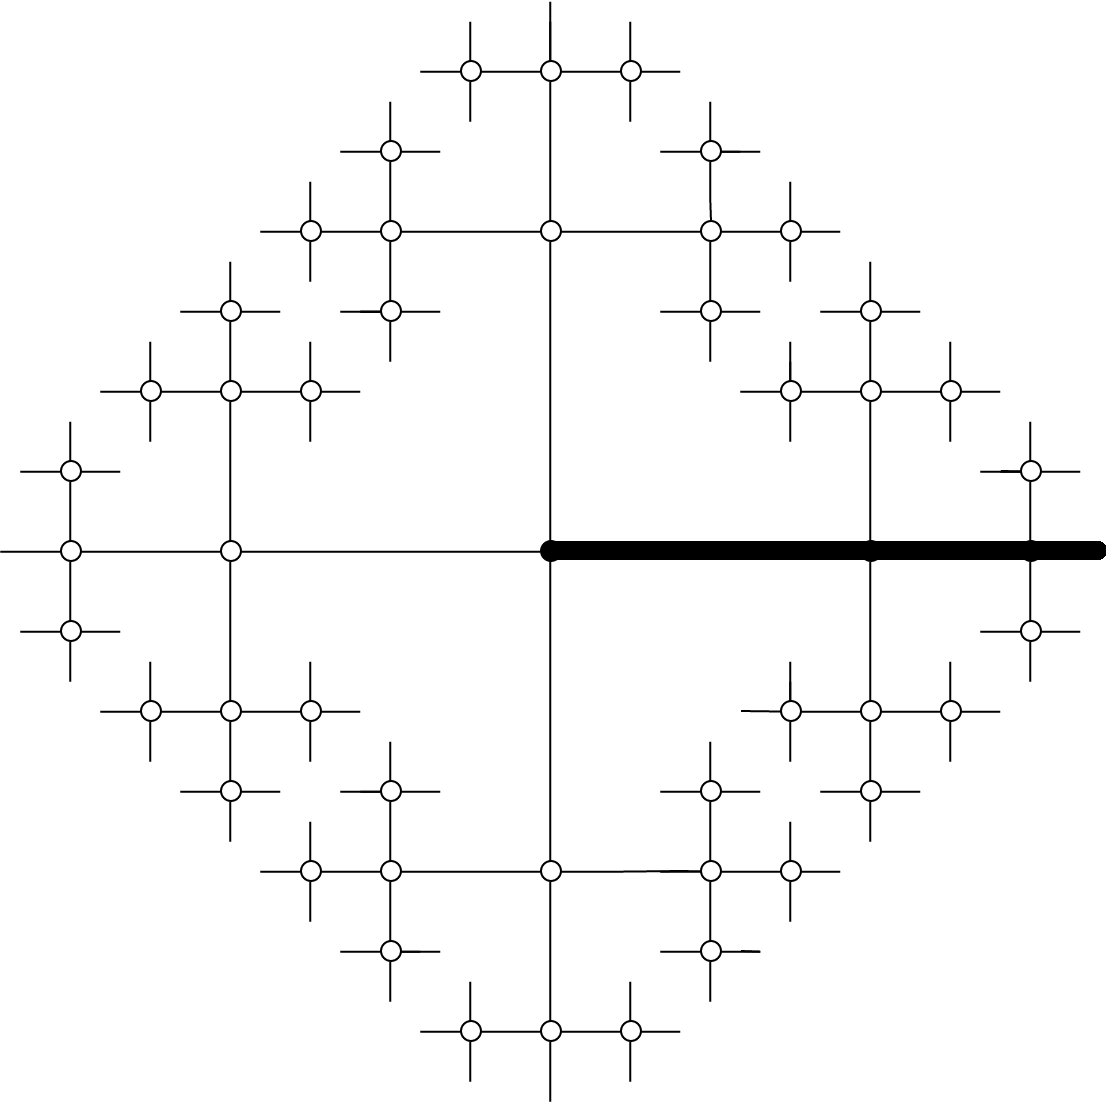
\includegraphics[width=6.5cm]{treeaaa.png}
          \caption{木aaa}
          \label{treeaaa}
        \end{center}
    \end{minipage}
      \begin{minipage}{0.5\hsize}
        \begin{center}
          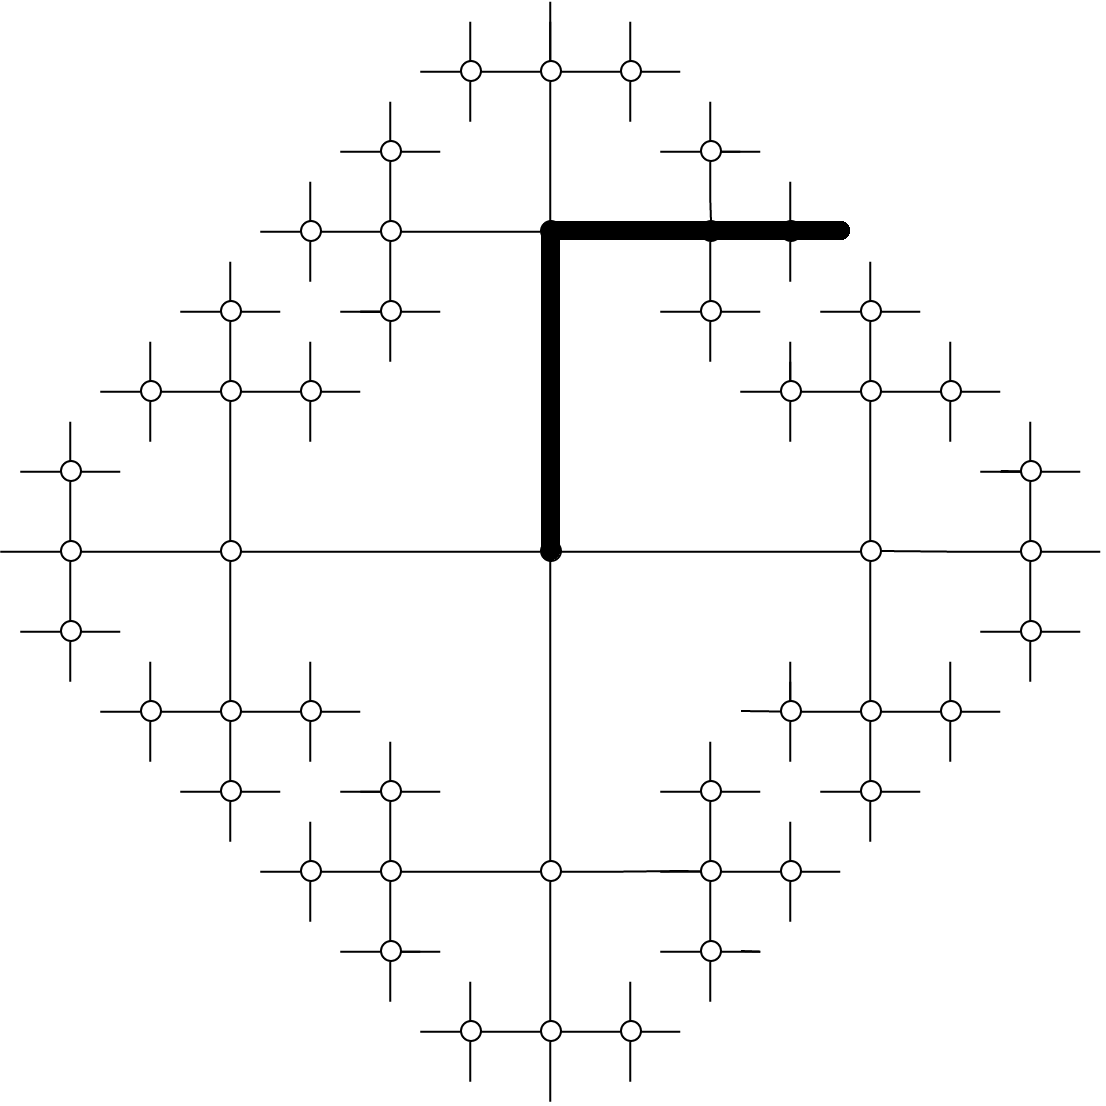
\includegraphics[width=6.5cm]{treebaa.png}
          \caption{木baa}
          \label{treebaa}
        \end{center}
      \end{minipage}
    \end{tabular}
    \end{center}
  \end{figure}
  ちなみに,木$T$には最短の道の長さを距離とする離散位相が入ります.
  次に,この木$T$の境界$\d T$を次のように,無限に続く既約な"語"の全体として定義する.
  \begin{align*}
    \d T := \{ x_1 x_2 x_3 \cdots | x_i \in S,\, 既約\}
  \end{align*}
  木$T$も境界$\d T$も右に語が続いているので,$\F_2$が左から作用することができます.
  例えば,$aaa\cdots \in \d T($図\ref{treeaaa}$)$に$b \in \F_2$を作用させると,$baaa\cdots \in \d T($図\ref{treebaa}$)$に移る.
  また,$\d T$には$\{U(v)\}_{v \in V(T)}$を開基とする位相が入ります.
  ただし,各頂点$v \in V(T)$に対し,
  \begin{align*}
    U(v) := \{ v x_1 x_2 x_3 \cdots | x_i \in S,\, 既約 \}
  \end{align*}
  と定めます.
  この位相により,$\d T$は完全不連結コンパクトハウスドルフ空間になります.
  ちなみに,この開基はコンパクト開集合です.
  \begin{proposition}
    $\d T$は$\F_2$-境界であり,$\F_2$は$\d T$にtopologically\, freeに作用する.
  \end{proposition}
  \begin{proof}
    まず,$\F_2$-境界であることを示す.
    
    1つ目に,minimalを示す.
    任意に$x = x_1x_2x_3 \cdots, y = y_1y_2y_3 \cdots \in \d T$をとる.
    $x_k = (y_1 y_2 \cdots y_k)(x_1 x_2 \cdots x_k)^{-1}x$と定めると,$y$に収束する.
    次に示す.
    開集合$U \ni y$を任意にとる.
    ある$n \in \N$があって,$U(y_1 y_2 \cdots y_n) \subset U$となるものがある.
    $k \leq n$に対して,$x_k \in U(y_1 y_2 \cdots y_n) \subset U$.

    2つ目に,strongly\, proximalを示す.
    任意に$\mu \in \P(\d T)$をとる.
    まず,ある$T$の頂点の列$y_k = x_1x_2 \cdots x_k$ $(x_i \in S)$で$\mu(U(y_k)) \rightarrow 0$であるものが存在する.
%    まず,ある$T$の頂点の列$y^{(j)}_k = x^{(j)}_1x^{(j)}_2 \cdots x^{(j)}_k$ $(x^{(j)}_i \in S, j \in \{1,2\})$で$\mu(U(x^{(j)}_k)) \rightarrow 0$であり,$U(x^{(1)}_k) \cap U(x^{(2)}_k) = \emptyset$となるものが存在する.
    %    さらに,$x^{(0)}_1 = a, x^{(1)}_1 = b$
    これは,$\mu(X) = \mu(U(a) \cup U(a^{-1})\cup U(b) \cup U(b^{-1})) =  \mu(U(a)) + \mu(U(a^{-1})) +  \mu(U(b)) + \mu(U(b^{-1}))$みたいな性質を用いて,区間縮小法と同様にして,実現できる.
    
    $y^{-1} = x_1^{-1}x_2^{-1}\cdots \in \d T$とし,
    $g_i = x_1^{-1}x_2^{-1} \cdots x_i^{-1} x_i^{-1} \cdots x_2^{-1}x_1^{-1}$とする.
%    $g_i = x_1x_2 \cdots x_i x_i \cdots x_2x_1$とする.
    %    $y_k.\mu \rightarrow \delta_{y^{-1}}$である.
    $\varepsilon > 0$と$f \in C(\d T)$をとる.
    $\{U(y_k^{-1})\}$が$y^{-1}$の基本近傍系をなすことから,ある$l_0 \in \N$があって,$|f(y^{-1}) - f(x)| < \varepsilon$ $(x \in U(y^{-1}_{l_0}))$となる.
    また,$y_k$の選び方から,ある$l_1 \in \N$があって,$\mu(U(y_{l_1})) < \min(\varepsilon, \varepsilon / \|f\|_{sup})$.
%    すると,ある$i_0$があって,任意の$i \geq i_0$に対して,$g_i^{-1}U(y_{l_1}^c) \subset U(y^{-1}_{l_0})$となるものがある.
    %    また,$\mu(g_i^{-1}U(y_{l_1}^c))= g_i.\mu(X-U(y_{l_1}))$
    
    よって,任意の$i \geq \max(l_0,l_1)$に対して,
    \begin{align*}
      \left|f(y^{-1}) - g_i.\mu(f)\right| &\leq \left|f(y^{-1}) - \int_{U(y_{l_1})^c}f(g_i.x) d\mu(x)\right| + \left|\int_{U(y_{l_1})}f(g_i.x) d\mu(x)\right|\\
      &\leq \left|f(y^{-1}) - \int_{U(y_{l_1})^c}f(y^{-1})d\mu\right| + \left| \int_{U(y_{l_1})^c}|f(y^{-1}) - f(g_i.x)|d\mu \right|+ \frac{\varepsilon}{\|f\|_{sup}}\cdot \|f\|_{sup}\\
      &\leq |f(y^{-1})|\mu(U(y_{l_1})) + \varepsilon\mu(\d T) + \varepsilon\\
      &\leq 3\varepsilon.
    \end{align*}

    次に,topologically\, freeを示す.
    $x = x_1x_2x_3 \cdots \in \d T$をとる.
    ある$e \neq g \in G$と$x$のある頂点$v \in U(v)$が存在して,$g|_{U(v)} = {\rm id}_{U(v)}$.
    しかし,$g$が固定する$\d T$の元は$ggg\cdots$と$g^{-1}g^{-1}g^{-1}\cdots$のみなので,
    矛盾する.
    よって,topologically\, freeである.
    この議論により,freeでないことも分かる.    
  \end{proof}
\end{example}
\begin{theorem}[\cite{furstenberg1973boundary}]
  離散群$G$に対して,普遍$G$-境界が存在する.
  つまり,任意の$G$-境界は普遍$G$-境界からの$G$-同変連続写像の像である.
\end{theorem}

\begin{definition}
  上の定理にある普遍$G$-境界をFurstenberg境界といい,$\d_F G$とかく.
\end{definition}

\section{$\d_F G = \d_H G$}
定理を述べるためにいくつか定義をする.
\begin{definition}
  C*-環の単位的自己共役閉部分空間をoperator\, systemといい,
  $G$作用を持つoperator\, systemを$G$-operator\, systemという.
  ただし,operator\, systemの自己同型写像はorder\, isomorphismとする.

  $\S\, \T$をoperator\, systemとし,
  $\varphi:\S \rightarrow \T$を$\C$-線形写像とする.
  $\varphi$が任意の$n \in \N$に対して,$\varphi\otimes {\id_{M_n(\C)}}$がpositiveであるとき,
  completely\, positiveという.特に,$\varphi$が単位元を保つなら,u.c.p.(unital\, completely\, positive)とかく.
  さらに,$G$-同変なら,$G$-u.c.p.とかく.
\end{definition}
次の定理がC*-単純性の証明において,重要な役割を果たす.
\begin{theorem}
  $\d_F G = \d_H G$.\\
  ただし,$d_H G$はHamana境界である.
\end{theorem}
これを使うことで,次に呪文を唱えることができるようになる.
$\S$をoperator\, systemとし,$\T$をそのoperator\, subsystemとする.
\begin{description}
\item[$G$-injectivity] 任意の$G$-u.c.p.写像$\varphi: \T \rightarrow C(\d_F G)$は$\S$上の$G$-u.c.p.写像に拡張される.
\item[$G$-essentiality] 全ての$G$-u.c.p.写像$\varphi: C(\d_F G) \rightarrow S$は等長である.
\item[$G$-rigidity] $C(\d_F G)$から自分自身への$G$-u.c.p.写像は${\rm id}_{C(\d_F G)}$のみである.
\end{description}
\begin{remark}
  $\ast$-準同型はcompletely\, positiveである.
\end{remark}
\section{C*-単純性}
この章ではC*-単純性の証明を行う.
準備として,いくつかの定理を述べる.
詳細は\cite{brown2008c}などを参照すると良い.
\begin{theorem}[Arveson's extension theorem]
  $A$を単位的C*-環とし,$\S \subset A$をoperator\, subsystemとする.
  このとき,任意のu.c.p.写像$\varphi:\S \rightarrow B(H)$は$A$上のu.c.p.写像に拡張される.
  ただし,$B(H)$はHilbert空間$H$上の有界線形作用素全体とする.
\end{theorem}

\begin{theorem}
  $A, B$をC*-環とし,$\varphi: A \rightarrow B$をu.c.p.写像とする.
  このとき,$a \in A$が$\varphi(a^*a) = \varphi(a)^*\varphi(a), \varphi(aa^*) = \varphi(a)\varphi(a)^*$を満たすとき,
  任意の$b \in A$に対して,$\varphi(ab) = \varphi(a)\varphi(b), \varphi(ba) = \varphi(b)\varphi(a)$が成立する.
\end{theorem}
\begin{definition}
  $\{a \in A|\varphi(a^*a) = \varphi(a)^*\varphi(a), \varphi(aa^*) = \varphi(a)\varphi(a)^*\}$を$\varphi$のmultiplicative\, domainという.
\end{definition}
\begin{definition}
  $A$を$G$-C*-環とする.
  このとき,$G$-u.c.p.写像$E : A \rtimes_r G \rightarrow A$で,
  \begin{align*}
    E(\sum_{g \in G\, fin.}a_g \lambda_g) = a_e
  \end{align*}
  であり,$E|_A = {\rm id}_A$
  となるものが唯一つ存在する.
  これをcanonical\, conditional\, expectationという.
\end{definition}
\begin{remark}
  canonical\, conditional\, expectationは忠実(i.e. $E(a^*a) = 0 \Rightarrow a = 0$)である.
\end{remark}
\begin{theorem}[\cite{Kalantar2017boundaries}]
  $G$を離散群とする.
  $\d_F G$を$G$のFurstenberg境界とする.
  このとき,次は同値である.
  \begin{enumerate}
  \item $G$はC*-単純性を持つ.
  \item 半直積C*-環$C(\d_F G) \rtimes_r G$が単純.
  \item ある$G$-境界$B$が存在して,半直積C*-環$C(B) \rtimes_r G$が単純.
  \item $G$の$\d_F G$への作用は(topologically)\, freeである.
  \item ある$G$-境界$B$が存在して,$G$の$B$への作用がtopologically\, freeである.
  \end{enumerate}
\end{theorem}
$4. \Rightarrow 1.$の証明のみ行う.この証明は\cite{breuillard2017c}を元にしている.
\begin{proof}
  $I$を$C_r^*(G)$の$0$でない両側閉イデアルとする.
  $\pi: C_r^*(G) \rightarrow B(H)$を商写像$C_r^*(G) \rightarrow C_r^*(G)/I$と$C_r^*(G)/I$のuniversal\, representationの合成とする.

  $\pi$が単射であることを示す
  ( $\Rightarrow$ $I \subset ${\rm ker}$(\pi) = 0 \, \Rightarrow I = 0$).
  
  Arveson's extension theoremより,あるu.c.p.写像$\varphi : C(\d_FG) \rtimes_r G \rightarrow B(H)$で$\varphi|_{C_r^*(G)} = \pi$となるものが存在する.
  $\varphi$が忠実であることを示せば良い
  ($\because$ $a \in {\rm ker}(\pi) \Rightarrow a^*a \in {\rm ker}(\pi) \subset {\ker \varphi} \Rightarrow a = 0$).
  ここで,$\pi$は$\ast$-準同型なので,$C_r^*(G)$は$\varphi$のmultiplicative\,domainに含まれる.
  特に,$a \in  C(\d_FG) \rtimes_r G$と$g \in G$に対して,
  \begin{align*}
    \varphi(\lambda_g a \lambda_g^*) = \varphi(\lambda_g) \varphi(a) \varphi(\lambda_g^*) =  \pi(\lambda_g) \varphi(a) \pi(\lambda_g^*) = {\rm Ad}(\pi(\lambda_g))\varphi(a)
  \end{align*}
  となる.
  つまり,$\phi$は$G$-同変になる.
  これで呪文を唱えることが可能になった.

  $G$-rigidityより,$\varphi|_{C(\d_F G)}$は等長である.
  よって,逆写像$(\varphi|_{C(\d_F G)})^{-1} : \varphi(C(\d_F G)) \rightarrow C(\d_FG)$が定義でき,これは$G$-u.c.p.写像になる.
  $G$-injectivityより,$G$-u.c.p.写像$\tau : {\rm Im}(\varphi) \rightarrow C(\d_F G)$で$\tau|_{\varphi(C(\d_F G))} = (\varphi|_{C(\d_F G)})^{-1}$となるものが存在する.
  \[
  \xymatrix{
    C(\d_F G)\rtimes G \ar[rr]^{\varphi} \ar@{.>}[d]^{\psi}& & {\rm Im}(\varphi)\ar@{}[d]|{\bigcup} \ar@{.>}[dll]^{\tau} \ar@{}[r]|*{\subset}&B(H) \\
    C(\d_F G) & & \varphi(C(\d_F G))  \ar[ll]^{(\varphi|_{C(\d_F G)})^{-1}}&
  }
  \]

  $\psi := \tau \circ \varphi :  C(\d_F G)\rtimes G \rightarrow C(\d_F G)$と定めると,
  これは$G$-u.c.p.写像の合成であるため,$G$-u.c.p.写像である.
  $\psi$がcanonical\, conditional\, expectation\, $E$と一致することを示す.
  これが分かると,canonical\, conditional\, expectationは忠実なので,$\varphi$も忠実なことが示される.
  $G$-rigidityより,$\psi|_{C(\d_F G)} : C(\d_F G) \rightarrow C(\d_F G)$は${\rm id}_{C(\d_F G)}$である.
  特に,$C(\d_F G)$は$\psi$のmultiplicative\, domainである.
  最後に,$e \neq s \in G$に対し,$\psi(\lambda_s) = 0$を示せば,canonical\, conditinal\, expectationとの一致が示される.
  $e \neq s \in G$をとる.
  $f \in C(\d_F G)$に対し,
  \begin{align*}
    \psi(\lambda_g)f = \psi(\lambda_g) \psi(f) = \psi(\lambda_gf) = \psi(\lambda_g f \lambda_g^* \lambda_g)
    = \psi(g.f \lambda_g) = g.f\psi(\lambda_g).
  \end{align*}
  特に,$G$はfreeに$\d_FG$に作用するので,$x \in X$に対して,$g.x \neq x$となる.
  よって,ある$f \in C(\d_F G)$が存在して,$f(x) \neq f(g.x)$となる.
  よって,$\psi(\lambda_g)(f(x) - f(g.x)) = 0$となり,
  $\psi(\lambda_g) = 0$が導かれる.
\end{proof}


\bibliographystyle{alpha}
\bibliography{santorini}
\end{document}
